\chapter{Konzept}
\label{chap:konzept}
\setcounter{footnote}{0}
Dieses Kapitel ist aus der Sicht des Datenflusses organisiert. Als erstes
gilt es die Daten zu beschaffen. Daraufhin werden sie verarbeitet und
der Frontendanwendung zugeliefert. Dort werden die Daten den Dashboards
und deren Diagrammen zugewiesen. In den Diagrammen werden die Daten
visualisiert. Zu guterletzt werden die Einstellungen der Dashboards
und die Zuweisung der Daten gespeichert.

Der zuvor beschriebene Vorgang geht bereits davon aus, dass die Daten im Backend
verarbeitet und daraufhin dem Frontend ausgeliefert werden. Die Arbeit entscheidet
sich hierfür aus drei Gründen. Sicherheit, Performanz und Flexibilität. Die URLs
zum Abrufen der Daten sollen im Client einstellbar sein. Würde man die Anfragen an
die externen APIs zur Beschaffung der Daten direkt aus dem Client heraus senden,
müssen bei allen externen APIs CORS-Header für die eigene Origin gesetzt sein \cite{CORSW3C}.
Des Weiteren bieten sich serverseitige Programmiersprachen besser zur Verhinderung
von Attacken zur Einschleusung von schädlichem Quellcode an.\footnote{Bei
Unmarshalling- und Validierungsverfahren ist Golang flexibler als das im Client ausgeführte JS.}
Für die Performanz sprechen folgende Gründe: Das Endgeräte des Clients ist womöglich
nicht zur Datenverarbeitung ausgelegt. Das mehrfache Berechnen der gleichen Anfrage
kann im Backend einfach abgefangen und aus dem Cache genommen werden. Die Verbindung
des Backendservers zur externen API ist in der Regel schneller als die Verbindung
des Clients zum Server. Wenn das Backend die Daten bereits Verarbeitet, wird nur noch
eine verdichtete Form der Daten an den Client gesendet.\footnote{Es ist davon auszugehen, dass
die aus der Verarbeitung resultierende Datenmenge geringer als die der initialen Anfrage ist.}
Für die Flexibilität spricht, dass die Verarbeitung so nicht in neue Frontendanwendungen
integriert werden muss.

Die Benutzerverwaltungslogik soll klar von der Datenbeschaffungs-, Verarbeitungs-
und Zulieferungslogik getrennt sein. Die Arbeit geht somit von zwei Services aus.
Dem \code{Resource Management Service}, der für die Verwaltung von Ressourcen wie Dashboards,
Diagrammen, Datenquellen und Benutzer zuständig ist, und dem \code{Data Delivery Service},
der sich um die zu analysierenden Daten kümmert.

Die folgenden Abschnitte gehen genauer in das Konzept der Gesamtanwendung ein.
In \Cref{sec:beschaffung} geht es um die Beschaffung der Daten. In \Cref{sec:verarbeitung}
wird ein Konzept zur Transformation der Daten in ein für die Diagramme plausibles Format
erarbeitet. In \Cref{sec:zulieferung} geht es um ein Konzept, das
eine leistungsfähige Datenauslieferung an die Clients ermöglicht. In \Cref{sec:andordnungundzuweisung}
geht es um die Erstellung Eines Dashboards und dessen Zuweisung auf die
Datenquellen. In \Cref{sec:darstellung} wird ein Konzept entwickelt,
was Daten möglichst flexibel im Client visualisieren kann.
Zu guterletzt wird in \Cref{sec:speicherung} die Speicherung der Dashboards behandelt.

\section{Beschaffung}
\label{sec:beschaffung}
Die Datenbeschaffung selbst behandelt das Verfahren, zu analysierende Daten
von einer externen API zu dem \code{Data Delivery Service} zu transportieren.
Hier bieten sich Open Source Message Broker wie RabbitMQ und Apache Kafka an.
Aktuell stellt GBO Datacomp hierfür allerdings eine REST-API zur Verfügung.
Für den Datentransport von der REST-API zu dem \code{Data Delivery Service} reicht somit
eine GET-Anfrage aus.

\section{Verarbeitung}
\label{sec:verarbeitung}
Die Verarbeitung der Daten ist ein komplexes Verfahren. Die bereits in der
Anforderungsanalyse erwähnt, liefert die API von GBO Datacomp die Daten im
JSON-Format aus. Die Arbeit entscheidet sich zur Datenverarbeitung für die
Verwendung einer Abfragesprache. In \Cref{chap:analysebestehendersoftwareloesungen}
wurden drei bestehende Softwarelösungen im Bereich der Datenvisualisierung von
Betriebsdaten analysiert. Dabei verwendete jede der Lösungen eine Abfragesprache,
um komplexere Datentransformationen durchzuführen. Bei der Implementierung einer
GUI zur Definition der Verarbeitungsweise der Daten kommt man schnell an seine Grenzen.
Die Möglichkeit, Felder aus verschiedenen Ebenen einer JSON-Datei auszuwählen
und in eine gewollte Ausgangsstruktur zu transformieren, ist mithilfe einer GUI nahezu
unmöglich. Außerdem ist mit einer Abfragesprache auch um einiges schneller als mit
der Verwendung einer GUI. Allerdings benötigt die Verwendung einer Abfragesprache
Einarbeitungszeit. Nichtsdestotrotz ist es für die Arbeit die einzige Möglichkeit,
die Flexibilität für die Datenverarbeitung sowie die Datenmodellierung der Daten
beizubehalten.

Softwarelösungen wie Power BI, Qlik und Tableau verwenden SQL-ähnliche Abfragesprachen.
Da die Eingangsdaten im JSON-Format vorliegen und das Frontend in JS geschrieben wird,
ist es naheliegend, eine JSON-Abfragesprache für die Arbeit zu verwenden. Die Arbeit
verwendet hierfür die JSON-Abfragesprache \code{JMESPath}.\footnote{http://jmespath.org/}
Die Abfragesprache wurde von James Saryerwinnie ins Leben gerufen und wird aktuell von
Amazon in ihrer Amazon Web Services CLI verwendet.\cite{AWSJMESPath} Eine Umsetzung von
\code{JMESPath} gibt es in Golang als auch in JS. Somit ist es möglich, die Daten im
Frontend sowie Backend zu verarbeiten. Die Idee ist es, den Benutzern die Verarbeitung
im Frontend zu ermöglichen. Dort kann der Benutzer die Daten passend verarbeiten und die
gewollte Abfragezeichenfolge abspeichern. Diese wird dann bei der Darstellung des 
Dashboards in der Datenanfrage an die \code{Data Delivery API} mitgesendet.
Die weitere Verarbeitung findet dann im Backend statt.

\begin{listing}[]
    \inputminted{jsx}{snippets/json/jmespath-example/jmespathinput.json}
    \caption{JMESPath Eingangsdaten}
    \label{lst:jmespatheingangsdaten}
\end{listing}

\begin{listing}[]
    \inputminted{jsx}{snippets/json/jmespath-example/jmespathquery.txt}
    \caption{JMESPath Abfrage}
    \label{lst:jmespathabfrage}
\end{listing}

\begin{listing}[]
    \inputminted{jsx}{snippets/json/jmespath-example/jmespathoutput.json}
    \caption{JMESPath Ausgangsdaten}
    \label{lst:jmespathausgangsdaten}
\end{listing}

Um die Datenverarbeitung mithilfe von \code{JMESPath} zu verdeutlichen, folgt ein
Beispiel: Das Array in Quellcode \ref{lst:jmespatheingangsdaten} beinhaltet zwei Ressourcen;
\code{Maschine 1} und \code{Maschine 2}. Es repräsentiert die durch die REST-API empfangenen
Daten.\footnote{Die Beispieldaten wurden simplifiziert.} In Quellcode \ref{lst:jmespathabfrage}
sieht man eine Abfrage, anhand welcher die Daten Verarbeitet werden. In Quellcode \ref{lst:jmespathausgangsdaten}
sieht man das Endresultat der Abfrage. Die Werte der Felder \code{name}, \code{performance} und \code{quality}
wurden mithilfe des Array-Selektor \code{[]} und des angehangenen Feldnamen ausgewählt.
Das Format der Datenausgabe ist ein gültiger Datensatz für die Diagrammvisualisierungsbibliothek
\code{chart.js}. Somit lassen sich die Eingangsdaten mithilfe eines sehr flexiblen Verfahrens
in verwendbare Ausgabedaten transformieren.

\section{Zulieferung}
\label{sec:zulieferung}
Das Konzept der Zulieferung der Daten ist in drei Abschnitte
unterteilt. In \Cref{subsec:datenuebermittlungskonzept} wird das Datenübermittlungskonzept
zwischen dem Client und dem \code{Data Delivery Service} vorgestellt.
In \Cref{subsec:echtzeitauslieferung} geht es um die Liveübertragung der Daten. In
\Cref{subsec:caching} wird ein Konzept zur Leistungssteigerung der Datenauslieferung
erarbeitet.

\subsection{Datenübermittlungskonzept}
\label{subsec:datenuebermittlungskonzept}
Zur Datenübermittlung verwendet die Arbeit das Publish/Subscribe Architekturkonzept.
Um die bidirektionale Kommunikation zwischen dem Client und dem Server zu ermöglichen,
wird das WebSocket-Protokoll verwendet. Verglichen mit HTTP ist das WebSocket-Protokoll
aufgrund der fehlenden Header-Fixkosten performanter. Eine aufrechterhaltene WebSocket-Verbindung
benötigt allerdings auch mehr Rechenleistung als einzelne Mitteilungen über HTTP. Des Weiteren
kann HTTP nur bedingt mithilfe von Server-Sent Events eine bidirektionale Verbindung aufbauen.
Server-Sent Events selbst sind allerdings nur unidirektional \cite[2. Abschnitt]{WebSocketVSSSE}.

\begin{figure}
    \begin{center}
    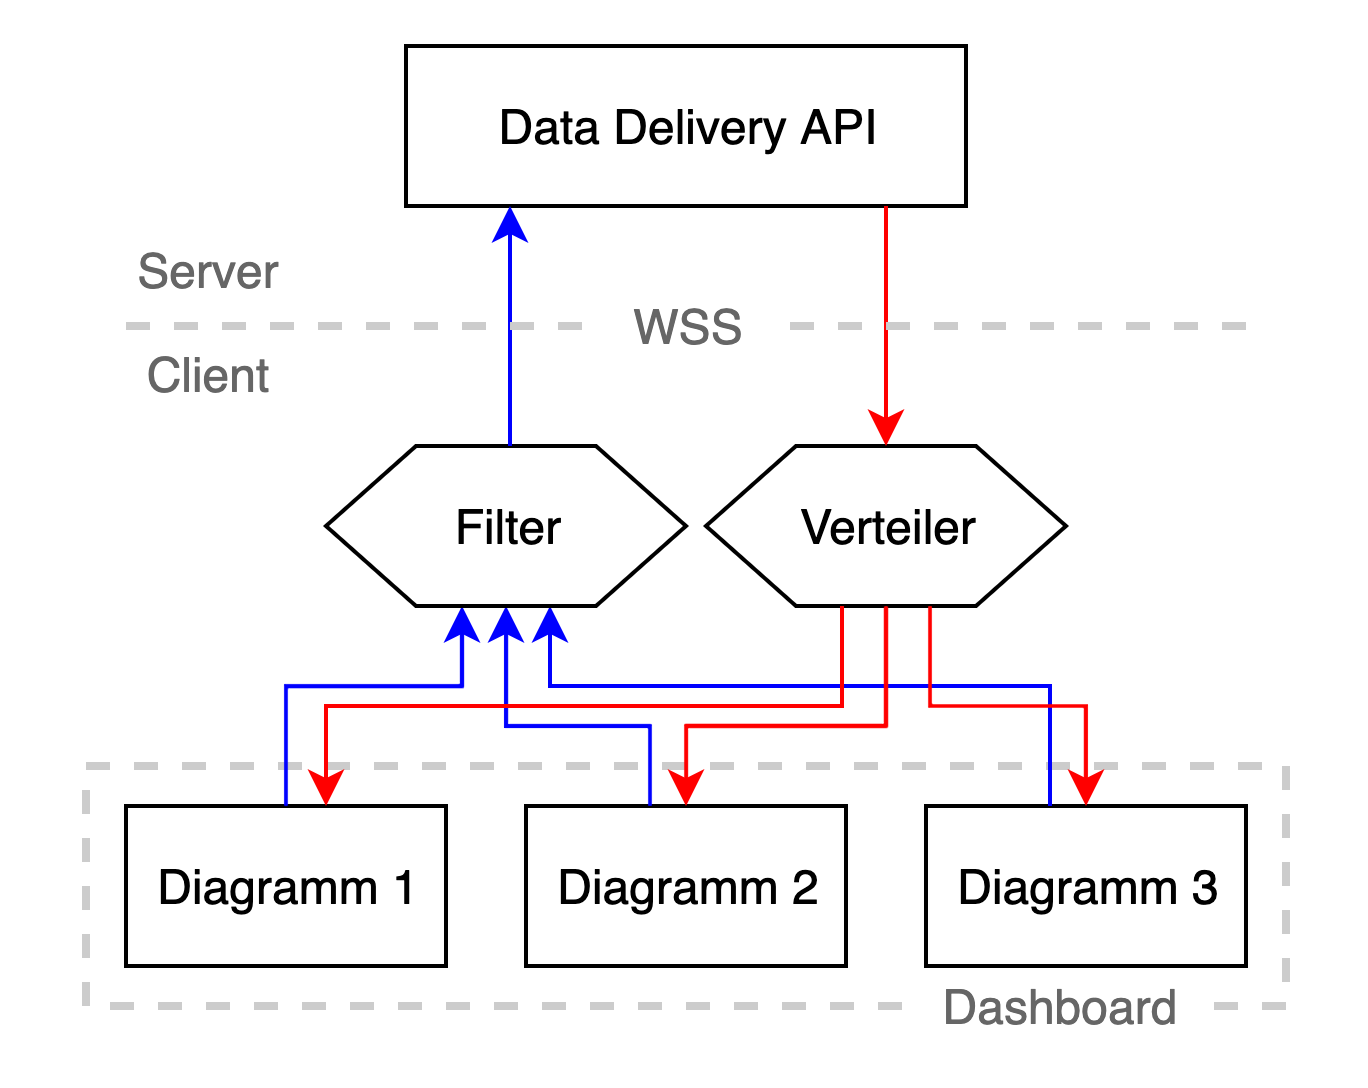
\includegraphics[scale=0.2]{img/abbildungen/Verteilung}
    \end{center}
    \caption{Verringerung der Redundanz des Datenflusses}
    \label{figure:uebersichtderdatenauslieferung}
\end{figure}

Das Konzept der Datenübermittlung ist Folgendes: Besucht der Nutzer ein Dashboard,
abonnieren die einzelnen Diagramme die jeweiligen Kanäle, die die Datenquellen 
repräsentieren (Siehe Abbildung \ref{figure:uebersichtderdatenauslieferung}).
Außerdem wird eine Nachricht an den \code{Data Delivery Service} veröffentlicht,
indem dieser darüber informiert wird, dass der Client jetzt bereit ist Daten zu empfangen.
Je nach angefragtem Interval sendet nun der \code{Data Delivery Service} verarbeitete
Daten an das Frontend, die in der Frontendanwendung angezeigt werden. Um die
Redundanz im Datenfluss zu verringern, werden die ausgehenden Nachrichten
so gefiltert, dass für jede Datenquelle nur eine Nachricht versendet wird. Die ankommenden
Nachrichten werden hingegen so verteilt, dass alle Diagramme mit der passenden Datenquelle
versorgt werden.

\subsection{Echtzeitauslieferung}
\label{subsec:echtzeitauslieferung}
Durch das Publish/Subscribe Architekturkonzept ist die Grundlage für die Echtzeitauslieferung
bereits geschaffen. Die im Dashboard enthaltenen Diagramme warten auf ankommende Nachrichten,
mit derer enthaltenen Daten sie ihre Visualisierung neuzeichnen. Der \code{Data Delivery Service}
benötigt eine in einem separaten Prozess taktierte Ausführung einer Routine, die die Daten
anhand eines gegebenen Intervals anfragt, verarbeitet und an die Frontendanwendung sendet.

\subsection{Caching}
\label{subsec:caching}
Der initiale Lade-, Verarbeitungs- und Auslieferungsprozess kann eine für den Benutzer
unangenehme Zeit in Anspruch nehmen. Um das initiale Warten beim Laden eines Dashboards
zu verringern, bietet sich folgende Caching-Strategie an: Bei einer Anfrage schaut
der \code{Data Delivery Service} zuerst, ob es bereits einen Cache-Eintrag für die
angefragte ID der Datenquelle gibt. Existiert dieser, wird eine sofortige Nachricht
mit den Daten aus dem Cache an die Frontendanwendung geschickt. Existiert anfangs noch
kein Cache-Eintrag, wird dieser Schritt übersprungen. Daraufhin werden
die aktuellen Daten in einem separaten Prozess abgefragt, verarbeitet, der Cache
aktualisiert und eine zweite Nachricht mit den aktuellen Daten an die Frontendanwendung
geschickt. Der Key für den Cache-Eintrag soll hierbei aus der ID der Datenquelle sowie
einem aus dem Request-Body generierten Hash zusammengesetzt werden. Somit werden
Kollisionen zwischen unterschiedlichen Benutzern ausgeschlossen\footnote{Die ID der Datenquellen ist
unter allen Nutzern einzigartig und wird dem Ersteller der Datenquelle zugewiesen.}
und Änderungen in dem Request-Body erkannt. Kollisionen unterhalb verschiedener
Benutzer könnten fatale Folgen haben. Im schlimmsten Fall würden so geheime Daten
in die Hände eines fremden Nutzers gelangen. Daher ist die Integration der Datenquellen-ID
in den Cache-Key essentiell.

\section{Anordnung und Zuweisung}
\label{sec:andordnungundzuweisung}
Das Konzept der Anordnung und Zuweisung ist in zwei Abschnitte unterteilt.
In \Cref{subsec:diagrammanordnungsverfahren} geht es um die Konzeptentwicklung
der Anordnung der Diagramme innerhalb eines Dashboards. Daraufhin geht
es in \Cref{subsec:zuweisungungvondatenquellen} um die Zuweisung der Datenquellen
zu den angeordneten Diagrammen.

\subsection{Diagrammanordnungsverfahren}
\label{subsec:diagrammanordnungsverfahren}
Das Diagrammanordnungsverfahren beschreibt den Prozess, einzelne Diagramme in einem Dashboard anzuordnen.
Um das Verfahren zu vereinfachen, ist ein automatisches Anordnen der Diagramme diagonal sowie vertikal vorgesehen.
Die Anordnung der einzelnen Diagramme soll mithilfe der FlexBox Technologie implementiert werden.
\footnote{CSS Flexible Box Layout, bekannt als FlexBox, ist ein standardisiertes Anordnungsmuster, das von allen gängigen Browsern unterstützt wird.\cite{CanIUseFlexBox}}
Im mobilen Format sollen die einzelnen Diagramme untereinander aufgelistet werden. 

\begin{figure}
    \begin{center}
    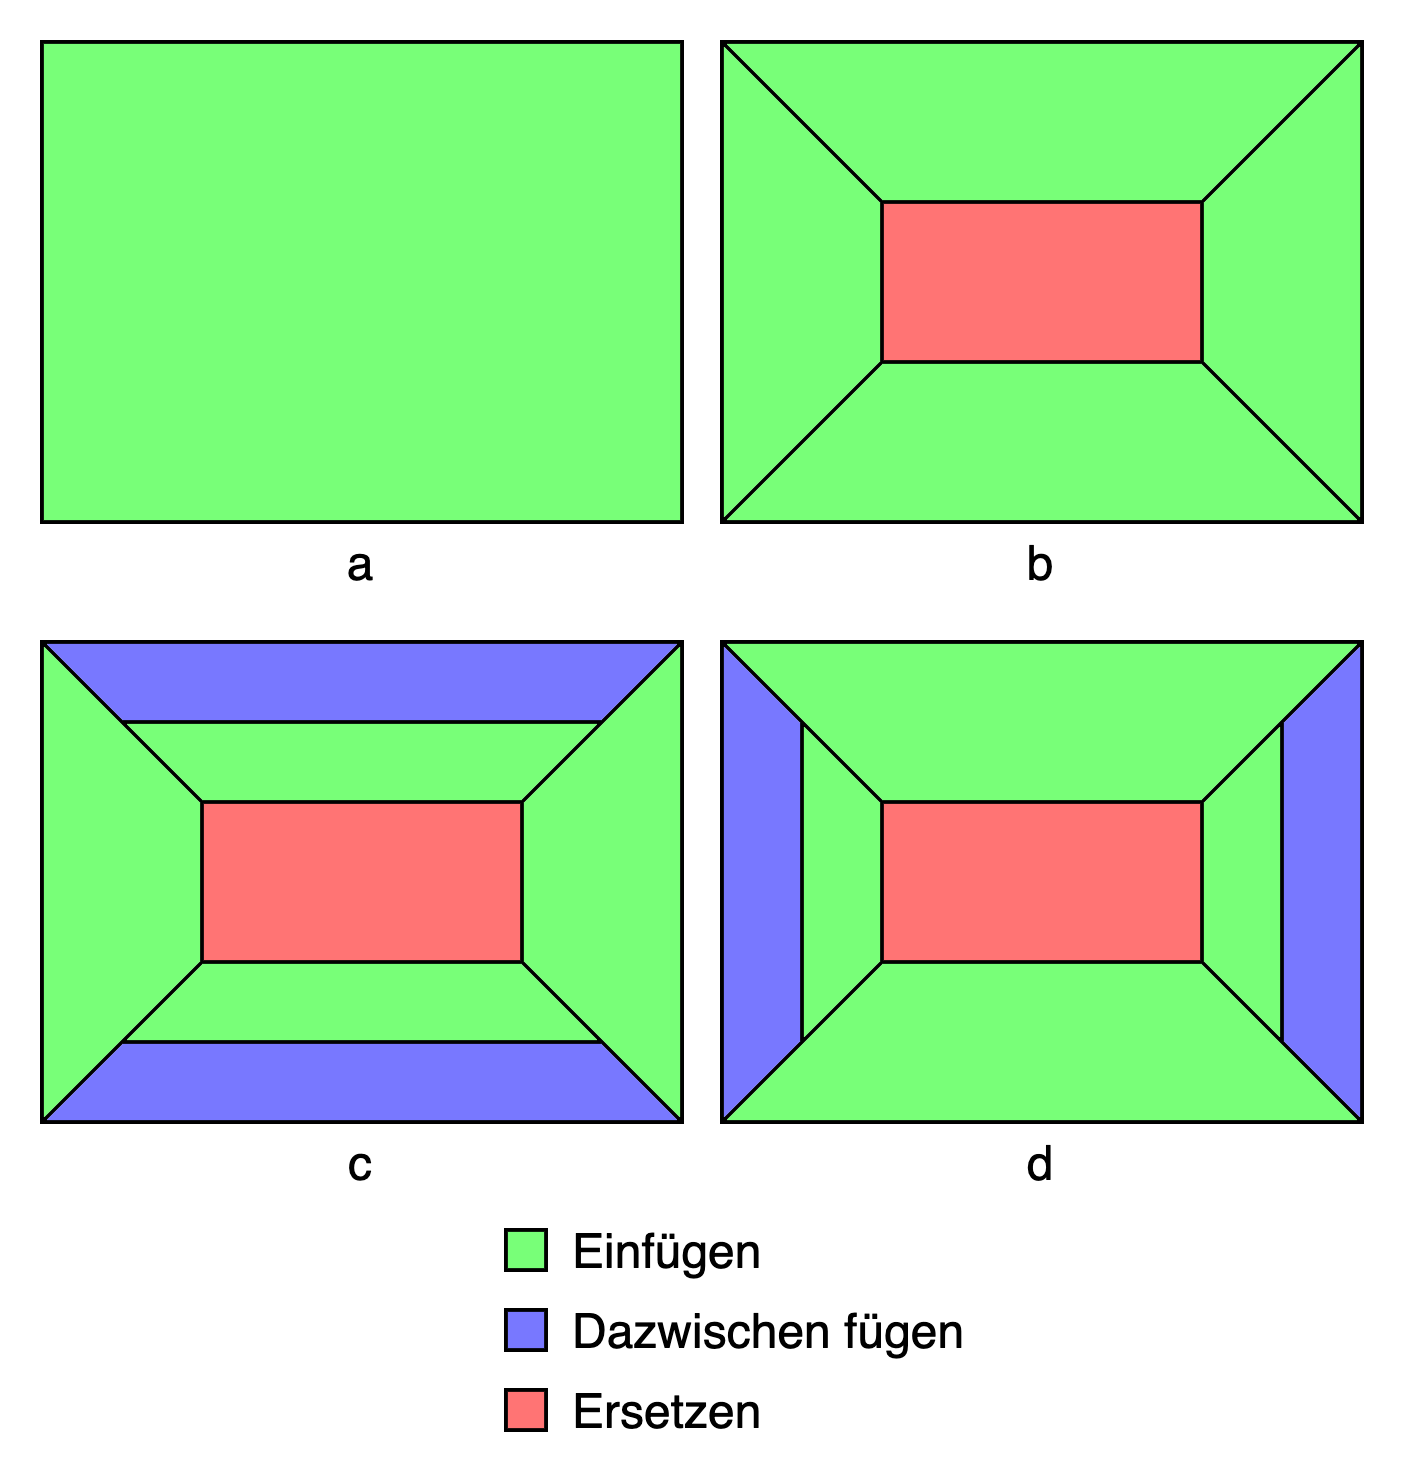
\includegraphics[scale=0.2]{img/abbildungen/DiagrammanordnungsverfahrenMitLegende}
    \end{center}
    \caption{Diagrammanordnungsverfahren}
    \label{figure:diagrammanaordnungsverfahren}
\end{figure}

Die Diagramme sollen nach und nach per Drag and Drop in das Dashboard integriert werden. Dieses Verfahren
wird in Abbildung \ref{figure:diagrammanaordnungsverfahren} dargestellt. \(a\) beschreibt den
initialen Zustand eines leeren Dashboards. Hier kann man durch Drag and Drop das erste Diagramm dem Dashboard
zuordnen. \(b\) beschreibt den Zustand des Dashboards mit genau einem enthaltenen Diagramm. Hier kann man das
neue Diagramm in alle Richtungen einfügen. Dabei Teilt das bestehende Diagram den Platz mit dem neuen gleichmäßig
auf. Bei der mittigen Positionierung wird das vorhandene Diagramm durch das neue ersetzt. \(c\) und \(d\)
beschreiben den Zustand, bei dem sich mehr als ein Diagramm im Dashboard befindet. Wenn man im Zustand \(b\)
ein Diagramm oberhalb oder unterhalb einfügt, bilden die beiden Diagramme eine Spalte. Beide dieser Diagramme
beinhalten nun den Zustand \(c\). Additional zu den möglichkeiten von Zustand \(b\), kann hier ein Diagramm
auch dazwischen gefügt werden. Es teilt sich dann den Platz mit den anderen Diagrammen in der Spalte.
Fügt man bei Zustand \(b\) ein Diagramm links oder rechts ein, bilden die beiden Diagramme eine Reihe.
Beide dieser Diagramme befinden sich nun in Zustand \(d\). Additional zu Zustand \(b\) können hier nun
auch neue Diagramme in der gleichen Reihe positioniert werden. Diese Reihen und Spalten können sich
immer weiter verschachteln. Somit kann der Benutzer mit einem ziemlich einfachen, intuitiven Verfahren
das Dashboard mit Diagrammen füllen. Durch einen Button in der Ecke rechts oben im Diagramm-Fenster
können diese auch wieder gelöscht werden. Dabei verhalten sich die zuvor beschriebenen Verfahren rückläufig.

\subsection{Zuweisung von Datenquellen}
\label{subsec:zuweisungungvondatenquellen}
Genauso wie bei der Anordnung der Diagramme in \Cref{subsec:diagrammanordnungsverfahren} werden
auch die Datenquellen per Drag and Drop auf die Diagramme im Dashboard verteilt. Aus einem kleinen
Menü aus der unteren rechten Ecke soll man die Rubrik Datenquelle auswählen und diese dann auf
die Diagramme im Dashboard ziehen. Daraufhin öffnet sich ein Dialogfenster mit einer Suchfunktion,
die einem ermöglicht eine Datenquelle zu suchen und auszuwählen. Diagramme, die bereits eine
Datenquelle zugewiesen haben, sollen diese im Fall einer Neuzuweisung mit den neuen Datenquellen
ersetzen. Anders als bei dem Diagrammanordnungsverfahren gibt es bei der Datenquellenzuweisung
nur eine mögliche Zuweisungsoption innerhalb des Diagramms. Das tauschen der X- und Y-Achse kann
entweder über die Änderungen des Datenausgangs in einer Datenquelle, in der Werkzeugleiste über
dem jeweiligen Plugin oder innerhalb des Plugins selbst ermöglicht werden.

\section{Darstellung}
\label{sec:darstellung}
Das Konzept der Darstellung der Frontendanwendung ist in zwei Abschnitte untergliedert.
In \Cref{subsec:zentralisierungderindividualisierbarkeit} wird ein Konzept für die
zentralisierte Anpassung der Benutzeroberfläche erarbeitet. In \Cref{subsec:pluginverfahren}
geht es um die ausgliederung der Gestaltung der einzelnen Diagramme aus der Frontendanwendung.
Somit soll mehr Flexibilität für die Umsetzung der einzelnen Diagramme geschaffen werden.
Gleichermaßen soll die Komplexität der Frontendanwendung gering gehalten werden.

\subsection{Zentralisierung der Individualisierbarkeit}
\label{subsec:zentralisierungderindividualisierbarkeit}
Für die Darstellung der Frontendanwendung wird das CSS-Framework Bootstrap verwendet.\footnote{https://getbootstrap.com/}
Die unkompilierte Form von Bootstrap ist in SASS geschrieben \cite[2. Abschnitt]{Bootstrap4punkt4}.
Die Arbeit verfolgt den Ansatz, für die Individualisierbarkeit relevante Parameter an einem Ort
zu zentralisieren. Diese Parameter sollen die Einstellungen von Bootstrap überschreiben und
in eigene SASS- sowie JS-Dateien importiert und verwendete werden. Somit kann mit der Veränderung
eines einzelnen Parameters die komplette Darstellung der Frontendanwendung angepasst werden.
WebPack, ein statischer Modulebündler für JS, ermöglicht mithilfe des \code{sass-loader}\footnote{https://www.npmjs.com/package/sass-loader} Variablen
aus SASS zu exportieren und daraufhin in JS zu importieren \cite{ShareSCSSwithJS}.

\subsection{Pluginverfahren}
\label{subsec:pluginverfahren}
% Bündelung der Bibliotheken

Die Arbeit verfolgt auch für das Frontend einen Microservice-Ansatz. Man spricht hier von einem
Microfrontend. Michael Geers schreibt dazu in einem Artikel auf Digital Pioneers Folgendes:

\begin{quote}
"Der Ansatz, der sich jetzt förmlich aufdrängt, ist die Umsetzung der Microservice-Idee
auch im Frontend. Anstatt einer ­großen Single-Page-Applikation baut man mehrere unabhängige
Teilapplikationen, die miteinander kommunizieren. Diese sind dann deutlich einfacher zu verstehen.
Der Einsatz einer neuen Technologie lässt sich in einem kleineren Rahmen testen."\cite{MicrofrontendT3N}
\end{quote}

Dabei sollen die Diagramme eines Dashboards als einzelne Services ausgelagert werden.
Die Diagramme können so einzeln entwickelt und ausgeliefert werden. Aufgrund der
gleichen Machenschaft der Schnittstellen der Diagramme, kann man diese Art des Code-Splittings auch als
einen Plugin-Ansatz ansehen. Die Diagramme sollen über die In-Memory-Datenbank
Redis zur Verfügung gestellt werden. Die Diagramme werden mithilfe
von Dynamic Imports\footnote{Dynamic Imports gibt es seit ES6 (ECMAScript 2015) \cite{DynamicImportsV8}}
während der Laufzeit agil nachgeladen. Da immer nur die verwendeten Diagramme aus der In-Memory-Datenbank
geladen werden, kann die Webanwendung eine nahezu unendliche Auswahl an möglichen Diagrammen zur Visualisierung
der Daten bereitstellen.

Verwendete Bibliotheken können in die Plugins integriert werden. Somit ist es möglich, für die Visualisierung
der Daten alle möglichen JS-Bibliotheken zu verwenden. So können Teile des Dashboards
in \code{chart.js}\footnote{https://www.chartjs.org/} und andere Teile in \code{d3.js}\footnote{https://d3js.org/}
umgesetzt werden. Die Bibliotheken selbst befinden sich nicht in der Frontendanwendung selbst,
sondern werden während der Laufzeit für die Diagramme, die diese verwenden, nachgeladen.
Ein Problem hierbei ist, dass durch das Bündeln der Diagramme in Module, die Bibliotheken für jedes einzelne
Modul gebündelt werden müssen. Somit werden bei einem Dashboard mit einer großen Anzahl an verschiedenen
Diagrammen, Bibliotheken mehrfach geladen. Um dies weitestmöglich zu verhindern, aber dennoch die Flexibilität
der Pluginentwicklung zu gewährleisten, werden ähnliche Plugins in Bündeln zusammengefügt. Wenn ein solches
Bündel an Diagrammen \code{chart.js} als Bibliothek für die Umsetzung ihrer Diagramme verwendet, wird diese
Bibliothek nur einmal für das ganze Bündel geladen.

\section{Speicherung}
\label{sec:speicherung}
Das Konzept der Speicherung der Daten ist in zwei Abschnitte unterteilt.
In \Cref{subsec:aufbauundeinstellungenderdashboards} geht es um die Persistierung des Aufbaus und der
Einstellungen der Dashboards. Der \Cref{subsec:weiterespeichermechanismen} handelt
von der Speicherung der Datenquellen, von für die Benutzerverwaltung benötigte Daten
sowie jegliche weitere für die Anwendung relevante Speichermechanismen.

\subsection{Aufbau und Einstellungen der Dashboards}
\label{subsec:aufbauundeinstellungenderdashboards}
Das Konzept der Speicherung des Aufbaus der Dashboards sieht es vor, dass die Anordnung 
der Diagramme als Baumstruktur im JSON-Format in der Datenbank persistiert wird. Mithilfe eines
rekursiven Algorithmus soll durch die Baumstruktur gelaufen werden, um so die für das Dashboard
nötigen Komponenten zu erstellen.\footnote{Unter "Weitere Quellcodeabschnitte" findet man ein Beispiel
einer JSON-Datei, die die Einstellungen und die Anordnung eines Dashboards beinhaltet.}
Zwischen der Anordnung und den Einstellungen des Dashboards soll eine UUID\footnote{UUID ist ein universeller,
einzigartiger Identifikator, der zufällig generiert wird. Aufgrund der Größe
von 128-Bit ist eine Kollision sehr gering \cite{UUIDJavaSEDocs}.} 
je Diagramm als Verweis benutzt werden. Dieses Konzept der Trennung zwischen
der Anordnung und den Einstellungen des Dashboards soll verhindert, dass
alle Informationen in einer immer komplexeren Baumstruktur gespeichert werden.
Außerdem können so Änderungen in dem Aufbau getrennt von den Änderungen in der
Einstellungen erkannt und darauf reagiert werden. Bei der Verwendung eines
Frameworks wie React kann so unterschieden werden, ob nur einzelne Komponenten
oder der komplette Aufbau des Dashboards gerendert werden muss.

Die ID der zu einem Dashboard zugewiesenen Datenquelle wird in dem Einstellungen
des jeweiligen Diagramms gespeichert. Jedes Diagramm hat die Möglichkeit,
Einstellungen zu persistieren. So kann sich die Anwendung beispielsweise merken,
welche Filteroptionen der Benutzer in einem bestimmten Diagramm als letztes verwendet
hat. Des Weiteren kann ein Diagramm wie in \Cref{subsec:zuweisungungvondatenquellen} beschrieben,
Änderungen in der Werkzeugleiste vornehmen. Diese Änderungen
sollen auch in den Einstellungen des jeweiligen Diagramms gespeichert werden.

\subsection{Weitere Speichermechanismen}
\label{subsec:weiterespeichermechanismen}
Typische Felder wie die ID, das Erstellungsdatum, der Titel und die Beschreibung einer Ressource,
werden in einer Datenbank gespeichert. Dadurch ist die Option gegeben, alle
Ressourcen nach Erstellungsdatum zu sortieren. Die IDs der Ressourcen sind kompakt gehalten,
da diese in der URL angezeigt werden. Hier ist das Konzept Folgendes: Eine achtstellige ID,
welche Klein- sowie Großbuchstaben und Zahlen beinhalten kann, wird vom \code{Ressource Management Service}
generiert. Daraufhin wird in der Datenbank geschaut, ob diese bereits existiert. Wenn nicht,
wird diese als ID für die neue, anzulegende Ressource verwendet. Falls die ID bereits existiert,
wird eine neue generiert und das Verfahren fängt wieder von vorne an, bis eine einzigartige ID gefunden wird.

Die CRUD-Operationen sollen für jede Ressource über den \code{Ressource Management Service}
in Form einer REST-API zur Verfügung gestellt werden. Für die Repräsentation der Plugins
in der URL sollen Slugs\footnote{Von Menschen lesbare, aneinandergereihte Buchstaben, Worte, Binde- und Unterstriche,
die eine Ressource beschreiben \cite{SlugTermDjango}.} verwendet werden.
